% =====================================================================
% Ilustrações "como fazer" do guia de montagem (TikZ).
% Incluído por montagem_fisica.tex depois das cores e das bibliotecas.
% Cada \ilXxx desenha uma figura; a legenda fica no texto principal.
% =====================================================================

\tikzset{
  il/.style={font=\sffamily\scriptsize},
  rot/.style={font=\sffamily\scriptsize, align=center},
  cota/.style={{Stealth[length=1.6mm]}-{Stealth[length=1.6mm]}, thin, black!70},
  guia/.style={thin, black!55},
  seta/.style={-{Stealth[length=2.2mm]}, thick, critico},
  peca/.style={fill=mecanica!30, draw=mecanica!70!black},
  metal/.style={fill=black!18, draw=black!60},
  latao/.style={fill=orange!45!yellow, draw=orange!60!black},
  pcb/.style={fill=green!35!black!70, draw=black!70},
  pino/.style={circle, fill=black!65, inner sep=0pt, minimum size=1.1mm},
  furo/.style={circle, draw=black!35, inner sep=0pt, minimum size=0.9mm},
}


% inserto em corte: trapézio serrilhado, lado estreito para baixo (x e y da base, em mm)
\newcommand{\insertoem}[2]{%
  \fill[latao] (#1-3.1,#2) -- (#1+3.1,#2) -- (#1+3.6,#2+7) -- (#1-3.6,#2+7) -- cycle;
  \foreach \t in {1.2,2.6,4.0,5.4} \draw[orange!60!black] (#1-3.3,#2+\t) -- (#1+3.3,#2+\t+0.8);
  \fill[white] (#1-1.5,#2) rectangle (#1+1.5,#2+7);
  \draw[orange!60!black] (#1-1.5,#2) -- (#1-1.5,#2+7) (#1+1.5,#2) -- (#1+1.5,#2+7);}
% capacitor cerâmico: disco em (x,y) com pernas até dois pontos
\newcommand{\ceram}[4]{%
  \draw[black!80, thick] (#1,#2) -- #3 (#1,#2) -- #4;
  \fill[orange!70!yellow, draw=orange!60!black] (#1,#2) circle (2.1);}

% ---------------------------------------------------------------------
% Inserto térmico em 3 passos (corte)
\newcommand{\ilInserto}{%
\begin{tikzpicture}[il, x=1mm, y=1mm]
  \foreach \k/\tit in {0/{1. apoie o inserto, reto},1/{2. afunde com o ferro},2/{3. assente com algo plano}} {
    \begin{scope}[xshift=\k*44mm]
      \fill[mecanica!30] (0,0) rectangle (30,14);
      \fill[white] (12,5) rectangle (18,14.2);
      \draw[mecanica!70!black] (0,14) -- (12,14) -- (12,5) -- (18,5) -- (18,14) -- (30,14);
      \node[rot, text width=40mm] at (15,-4) {\tit};
    \end{scope}
  }
  % 1
  \insertoem{15}{14.3}
  \draw[seta] (24,22) node[right, black, align=left] {lado estreito\\para baixo} -- (18.5,17);
  % 2
  \begin{scope}[xshift=44mm]
    \insertoem{15}{9.5}
    \fill[metal] (13.4,16.5) -- (16.6,16.5) -- (18,24) -- (12,24) -- cycle;
    \fill[metal] (12.4,24) rectangle (17.6,38);
    \fill[mecanica!50] (11.4,14) -- (12,12.5) -- (12.6,14) -- cycle;
    \fill[mecanica!50] (17.4,14) -- (18,12.5) -- (18.6,14) -- cycle;
    \draw[seta] (24,34) -- (24,22);
    \node[right, align=left] at (25,30) {só o peso\\do ferro};
    \node[left, align=right] at (11,32) {ferro a\\\textbf{220~°C}};
  \end{scope}
  % 3
  \begin{scope}[xshift=88mm]
    \insertoem{15}{6.8}
    \fill[metal] (7,14.2) rectangle (23,19);
    \node at (15,16.6) {metal frio};
    \draw[seta] (15,26) -- (15,19.5);
    \node[right] at (16,24) {5~s};
    \draw[cota] (27,14) -- (27,13.8);
    \draw[guia] (23,13.8) -- (29,13.8);
    \node[right, align=left] at (28,9) {topo\\0,2~mm\\abaixo};
  \end{scope}
\end{tikzpicture}}

% ---------------------------------------------------------------------
% Ordem de aperto: 12 parafusos M8 e 4 parafusos M3
\newcommand{\ilAperto}{%
\begin{tikzpicture}[il]
  \fill[orange!30, draw=orange!70!black] (0,0) circle (1.75);
  \fill[white, draw=orange!70!black] (0,0) circle (0.5);
  \foreach \p/\n in {0/1,1/5,2/9,3/3,4/7,5/11,6/2,7/6,8/10,9/4,10/8,11/12}
    \node[circle, draw, fill=white, inner sep=0pt, minimum size=4.4mm,
      font=\sffamily\scriptsize\bfseries] (b\n) at ({90-(\p+0.5)*30}:1.25) {\n};
  \draw[seta, shorten <=2.4mm, shorten >=2.4mm, thin] (b1) -- (b2);
  \draw[seta, shorten <=2.4mm, shorten >=2.4mm, thin] (b3) -- (b4);
  \node[below, align=center] at (0,-1.9) {12 parafusos M8: siga os números\\(cada um seguido do oposto)};
  \begin{scope}[xshift=4.3cm]
    \fill[black!15, draw=black!60] (0,0) circle (0.95);
    \fill[white, draw=black!60] (0,0) circle (0.3);
    \foreach \a/\n in {45/1,225/2,135/3,315/4}
      \node[circle, draw, fill=white, inner sep=0pt, minimum size=4.4mm,
        font=\sffamily\scriptsize\bfseries] at (\a:0.62) {\n};
    \node[below, align=center] at (0,-1.9) {4 parafusos M3 do flange:\\em cruz};
  \end{scope}
\end{tikzpicture}}

% ---------------------------------------------------------------------
% Capacitores soldados no motor (vista da tampa de trás)
\newcommand{\ilCapMotor}{%
\begin{tikzpicture}[il, x=1mm, y=1mm]
  \fill[black!30] (0,0) circle (22);
  \fill[black!10, draw=black!50] (0,0) circle (18.5);
  \fill[black!22] (0,0) circle (5.5);
  % ponto lixado na carcaça
  \fill[pattern=north east lines, pattern color=black!70] (0,20.25) ellipse (3.2 and 1.6);
  \draw[black!70] (0,20.25) ellipse (3.2 and 1.6);
  % terminais
  \foreach \s in {-1,1} \fill[latao] (\s*10-1.6,6) rectangle (\s*10+1.6,15);
  \fill[critico] (13.5,15.5) circle (1.1);
  \node[font=\sffamily\bfseries] at (10,3.5) {$+$};
  \node[font=\sffamily\bfseries] at (-10,3.5) {$-$};
  \ceram{0}{9}{(-8.4,10)}{(8.4,10)}
  \ceram{6}{18}{(10,15)}{(2.6,20.3)}
  \ceram{-6}{18}{(-10,15)}{(-2.6,20.3)}
  % chicote
  \draw[line width=1.6pt, red!75!black] (10,6) -- (10,-8) -- (30,-8);
  \draw[line width=1.6pt, black] (-10,6) -- (-10,-11) -- (30,-11);
  \node[right] at (30,-9.5) {chicote trançado (M+ e M$-$)};
  % rótulos
  \draw[guia] (0,9) -- (-30,2) node[left, align=right] {C1: entre\\os terminais};
  \draw[guia] (-6,18) -- (-30,22) node[left, align=right] {C2 e C3: de cada\\terminal à carcaça};
  \draw[guia] (6,18) -- (-30,22);
  \draw[guia] (2,21.4) -- (24,28) node[right, align=left] {ponto lixado\\na carcaça};
  \draw[guia] (13.5,15.5) -- (28,17) node[right, align=left] {marca vermelha\\= terminal $+$};
\end{tikzpicture}}

% ---------------------------------------------------------------------
% Flange: posição no eixo e parafuso de trava no lado plano
\newcommand{\ilFlange}{%
\begin{tikzpicture}[il, x=1.9mm, y=1.9mm]
  % motor (atrás) e parede do braço
  \fill[black!25] (-11,-14) rectangle (-3.5,14);
  \node[rot] at (-7.3,0) {motor};
  \fill[peca] (-3.5,9.05) rectangle (0,14);
  \fill[peca] (-3.5,-14) rectangle (0,-9.05);
  \node[rot, mecanica!70!black] at (-1.75,16) {braço};
  % ressalto e eixo
  \fill[black!40] (-3.5,-8.75) rectangle (1.1,8.75);
  \fill[black!30, draw=black!60] (1.1,-2.5) rectangle (18.1,2.0);
  % flange: cubo e disco
  \fill[black!12, draw=black!60] (3,-5) rectangle (12,5);
  \fill[black!12, draw=black!60] (12,-11) rectangle (15,11);
  \fill[black!70] (6.6,2.0) rectangle (8.4,5.8);
  % roda (contorno)
  \draw[orange!70!black, dashed] (15,-13) rectangle (20,13);
  \node[rot, orange!70!black] at (17.5,15) {roda};
  % calço de 2 mm
  \fill[critico] (2.05,3.5) circle (0.95);
  \draw[guia] (2.05,4.4) -- (-1,22) node[above, align=center] {broca de 2~mm\\como calço};
  \draw[cota] (1.1,-7) -- (3,-7);
  \node[below] at (2.05,-7.6) {$\approx$2~mm};
  \draw[guia] (1.1,-2.5) -- (1.1,-8);
  \draw[guia] (3,-5) -- (3,-8);
  \node[rot] at (7.5,-15) {cubo do flange};
  \node[rot] at (13.5,13) {disco};
  \draw[guia] (7.5,5.8) -- (9,20) node[above, align=center] {parafuso\\de trava};
  % corte do eixo: lado plano
  \begin{scope}[xshift=34*1.9mm]
    \fill[black!12, draw=black!60] (0,0) circle (5);
    \fill[black!30, draw=black!60] (-1.5,2.0) -- (1.5,2.0) arc[start angle=36.9, end angle=-216.9, radius=2.5] -- cycle;
    \fill[black!70] (-0.9,2.0) rectangle (0.9,6.6);
    \fill[black!70] (2.5,-0.9) rectangle (6.6,0.9);
    \draw[seta] (0,10) -- (0,6.9);
    \node[above, align=center] at (0,10) {este no\\lado plano};
    \node[below, align=center] at (0,-6) {corte do cubo:\\eixo com um lado plano};
  \end{scope}
\end{tikzpicture}}

% ---------------------------------------------------------------------
% Pivô em corte: ordem das peças na barra e o calço de papel
\newcommand{\ilPivo}{%
\begin{tikzpicture}[il, x=1.45mm, y=1.45mm]
  % suportes da base
  \foreach \a/\b in {-21/-9, 43/55} {
    \fill[black!20, draw=black!55] (\a,-19) rectangle (\b,11);
    \fill[latao] ({(\a+\b)/2-2},6) rectangle ({(\a+\b)/2+2},11);
    \fill[black!65] ({(\a+\b)/2-0.8},4) rectangle ({(\a+\b)/2+0.8},12.5);
  }
  \fill[black!35] (-30,-19) rectangle (64,-21);
  % tubo do braço e rolamentos
  \fill[peca] (0,-16) rectangle (34,16);
  \fill[peca] (12,16) rectangle (22,24);
  \fill[peca] (14,-16) rectangle (20,-22);
  \foreach \a in {0,27} {
    \fill[black!15, draw=black!60] (\a,-11) rectangle (\a+7,11);
    \fill[black!40, draw=black!60] (\a,-6) rectangle (\a+7,6);
  }
  % colares
  \foreach \a in {-8,34} {
    \fill[black!30, draw=black!60] (\a,-7) rectangle (\a+8,7);
    \fill[black!70] (\a+3.2,7) rectangle (\a+4.8,9);
  }
  % barra
  \fill[black!45, draw=black!70] (-24,-4) rectangle (58,4);
  \draw[seta, line width=1.2pt] (-36,0) -- (-25,0);
  \node[above, align=center] at (-31,1) {a barra\\entra aqui};
  % ordem
  \foreach \x/\n/\t in {-15/1/{suporte\\da frente}, -4/2/colar, 17/3/{braço\\(2 rolamentos)}, 38/4/colar, 49/5/{suporte\\de trás}} {
    \node[circle, draw, fill=white, inner sep=0.6pt, font=\sffamily\scriptsize\bfseries] at (\x,33) {\n};
    \node[rot, below] at (\x,31) {\t};
  }
  \node[rot, text=orange!70!black] at (-15,-25) {frente\\(lado da roda)};
  \node[rot] at (49,-25) {trás\\(lado da bandeja)};
  \node[rot, text=white] at (17,-14) {tubo};
  \draw[guia] (49,12.5) -- (58,20) node[right, align=left] {trava da barra:\\M3 no topo}; 
  % detalhe do papel
  \draw[critico, thick] (-0.25,-6) -- (-0.25,6);
  \draw[guia] (-0.25,-5) -- (3,-33) node[below, align=center] {papel entre o colar e o anel interno do rolamento:\\aperte o colar e tire o papel};
\end{tikzpicture}}

% ---------------------------------------------------------------------
% Policarbonato e barra: medidas
\newcommand{\ilPoliBarra}{%
\begin{tikzpicture}[il, x=0.24mm, y=0.24mm]
  \fill[cyan!8, draw=cyan!50!black] (0,0) rectangle (230,230);
  \foreach \x in {55,175} {
    \draw[black, fill=white] (\x,20) circle (4);
    \draw[guia] (\x-8,20) -- (\x+8,20) (\x,12) -- (\x,28);
  }
  \draw[cota] (0,250) -- (230,250) node[midway, above] {230};
  \draw[cota] (-18,0) -- (-18,230) node[midway, left] {230};
  \draw[cota] (0,55) -- (55,55) node[midway, above] {55};
  \draw[cota] (55,55) -- (175,55) node[midway, above] {120};
  \draw[cota] (175,55) -- (230,55) node[midway, above] {55};
  \draw[guia] (55,24) -- (55,60) (175,24) -- (175,60);
  \draw[cota] (205,0) -- (205,20) node[midway, right] {20};
  \draw[guia] (175,20) -- (212,20);
  \node at (115,140) {policarbonato 2--3~mm};
  \node[align=center] at (115,100) {2 furos de \textbf{3,5~mm}\\(madeira por baixo, baixa rotação)};
  \node[below] at (115,-6) {borda de baixo: entra nas ranhuras dos postes};
  % barra
  \begin{scope}[xshift=300*0.24mm, yshift=110*0.24mm]
    \fill[black!30, draw=black!70] (0,0) -- (82*2-4,0) -- (82*2,4) -- (82*2,12) -- (82*2-4,16) -- (0+4,16) -- (0,12) -- (0,4) -- cycle;
    \draw[cota] (0,32) -- (164,32) node[midway, above] {\textbf{82~mm} (escala 2:1 no desenho)};
    \node[below, align=center] at (82,-6) {barra de 8~mm: corte, lime e\\faça um chanfro leve nas pontas};
  \end{scope}
\end{tikzpicture}}

% ---------------------------------------------------------------------
% Balanceamento da roda
\newcommand{\ilBalanceamento}{%
\begin{tikzpicture}[il]
  \foreach \k in {0,1} {
    \begin{scope}[xshift=\k*4.6cm]
      \fill[orange!30, draw=orange!70!black] (0,0) circle (1.4);
      \fill[white, draw=orange!70!black] (0,0) circle (0.45);
      \foreach \p in {0,...,11} \fill[black!45] ({90-(\p+0.5)*30}:1.05) circle (0.12);
    \end{scope}
  }
  \fill[critico] (-90+15:1.05) circle (0.17);
  \node[below, align=center] at (0,-1.6) {sempre para com o mesmo\\lado embaixo: lado pesado};
  \draw[seta] (-1.9,0.9) arc[start angle=150, end angle=210, radius=1.8];
  \begin{scope}[xshift=4.6cm]
    \fill[critico] (90-15:1.05) circle (0.17);
    \fill[black!45] (-90+15:1.05) circle (0.17);
    \draw[seta, bend left=50] (-90+15:1.25) to (90-15:1.25);
    \node[below, align=center] at (0,-1.6) {troque: o parafuso mais\\pesado vai para cima};
  \end{scope}
  \draw[-{Stealth[length=3mm]}, line width=1.4pt, black!50] (1.9,0) -- (2.7,0);
\end{tikzpicture}}

% ---------------------------------------------------------------------
% Placa de proteção do barramento (vista de cima)
\newcommand{\ilProtecao}{%
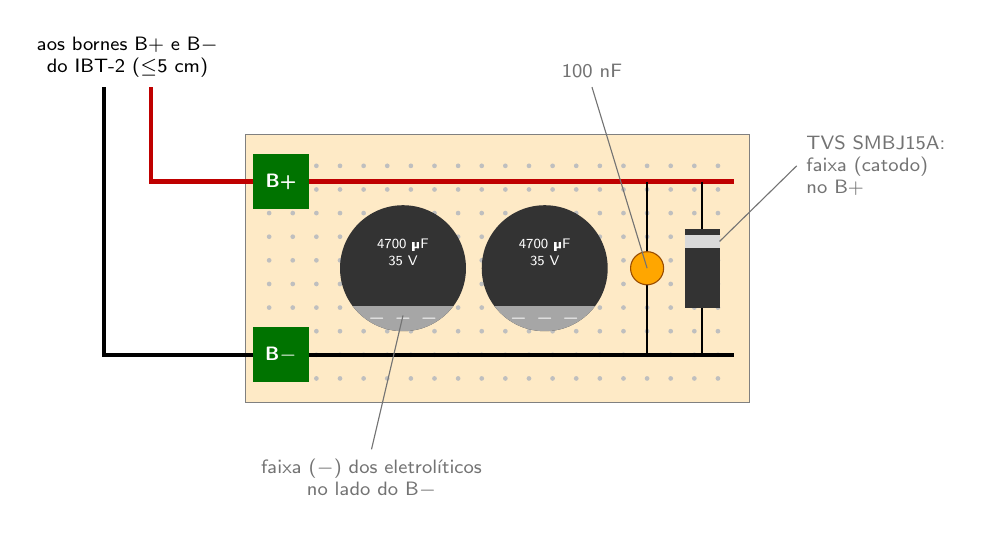
\begin{tikzpicture}[il, x=1mm, y=1mm]
  \fill[yellow!25!orange!20, draw=black!50] (0,0) rectangle (64,34);
  \foreach \x in {3,6,...,62} \foreach \y in {3,6,...,32} \fill[black!25] (\x,\y) circle (0.3);
  % barramentos
  \draw[line width=1.6pt, red!75!black] (8,28) -- (62,28);
  \draw[line width=1.6pt, black] (8,6) -- (62,6);
  % bornes
  \foreach \y/\t in {28/B+, 6/B$-$} {
    \fill[green!45!black] (1,\y-3.5) rectangle (8,\y+3.5);
    \node[white, font=\sffamily\scriptsize\bfseries] at (4.5,\y) {\t};
  }
  % eletrolíticos: faixa do lado do B-
  \foreach \x in {20,38} {
    \fill[black!80] (\x,17) circle (8);
    \begin{scope}
      \clip (\x,17) circle (8);
      \fill[black!35] (\x-9,9) rectangle (\x+9,12.2);
    \end{scope}
    \node[white] at (\x,10.6) {$-\,-\,-$};
    \node[white, align=center, font=\sffamily\tiny] at (\x,19) {4700~\textmu F\\35~V};
  }
  % cerâmico
  \draw[thick] (51,28) -- (51,6);
  \fill[orange!70!yellow, draw=orange!60!black] (51,17) circle (2.1);
  % TVS: faixa (catodo) do lado do B+
  \draw[thick] (58,28) -- (58,6);
  \fill[black!80] (55.8,12) rectangle (60.2,22);
  \fill[white!85!black] (55.8,19.6) rectangle (60.2,21.2);
  % rótulos
  \draw[guia] (20,11) -- (16,-6) node[below, align=center] {faixa ($-$) dos eletrolíticos\\no lado do B$-$};
  \draw[guia] (51,17) -- (44,40) node[above] {100~nF};
  \draw[guia] (60.2,20.4) -- (70,30) node[right, align=left] {TVS SMBJ15A:\\faixa (catodo)\\no B+};
  \draw[line width=1.6pt, red!75!black] (1,28) -- (-12,28) -- (-12,40);
  \draw[line width=1.6pt, black] (1,6) -- (-18,6) -- (-18,40);
  \node[above, align=center] at (-15,40) {aos bornes B+ e B$-$\\do IBT-2 ($\leq$5~cm)};
\end{tikzpicture}}

% ---------------------------------------------------------------------
% Ajuste do buck
\newcommand{\ilBuck}{%
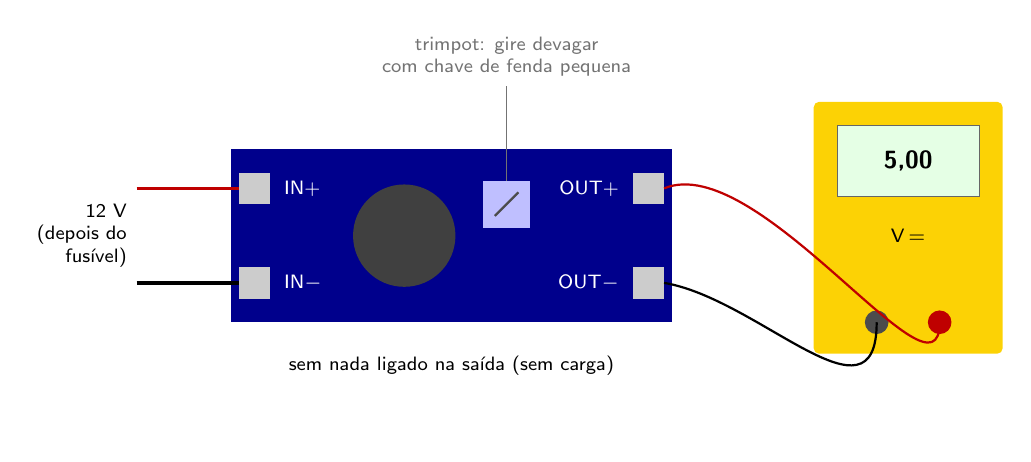
\begin{tikzpicture}[il, x=1mm, y=1mm]
  \fill[blue!55!black] (0,0) rectangle (56,22);
  \foreach \y/\t in {17/IN+, 5/IN$-$} {\fill[black!20] (1,\y-2) rectangle (5,\y+2); \node[white, right] at (5.5,\y) {\t};}
  \foreach \y/\t in {17/OUT+, 5/OUT$-$} {\fill[black!20] (51,\y-2) rectangle (55,\y+2); \node[white, left] at (50.5,\y) {\t};}
  \fill[black!75] (22,11) circle (6.5);
  \fill[blue!25] (32,12) rectangle (38,18);
  \draw[black!70, thick] (33.5,13.5) -- (36.5,16.5);
  \draw[guia] (35,18) -- (35,30) node[above, align=center] {trimpot: gire devagar\\com chave de fenda pequena};
  \draw[line width=1.2pt, red!75!black] (-12,17) -- (1,17);
  \draw[line width=1.2pt, black] (-12,5) -- (1,5);
  \node[left, align=right] at (-12,11) {12~V\\(depois do\\fusível)};
  \begin{scope}[xshift=74mm, yshift=-4mm]
    \fill[yellow!70!orange, rounded corners=2pt] (0,0) rectangle (24,32);
    \fill[green!10, draw=black!60] (3,20) rectangle (21,29);
    \node[font=\sffamily\bfseries\small] at (12,24.5) {5,00};
    \node at (12,15) {V$\,=$};
    \fill[black!70] (8,4) circle (1.5);
    \fill[red!75!black] (16,4) circle (1.5);
  \end{scope}
  \draw[red!75!black, thick] (90,0) .. controls (90,-12) and (67,22) .. (55,17);
  \draw[black, thick] (82,0) .. controls (82,-14) and (67,3) .. (55,5);
  \node[below, align=center] at (28,-3) {sem nada ligado na saída (sem carga)};
\end{tikzpicture}}

% ---------------------------------------------------------------------
% Pinagem da Black Pill (WeAct V3.x, vista de cima, USB-C à esquerda)
\newcommand{\ilBlackPill}{%
\begin{tikzpicture}[il, x=1mm, y=1mm]
  \fill[blue!65!black, rounded corners=1pt] (0,0) rectangle (60,21);
  \fill[black!25, draw=black!60] (-3,7) rectangle (5,14);
  \node[rot, font=\sffamily\tiny] at (1,10.5) {USB-C};
  \fill[black] (25,7.5) rectangle (32,13.5);
  \node[white, font=\sffamily\tiny] at (28.5,10.5) {F411};
  \foreach \y/\t in {16.5/KEY, 4.5/NRST} {\fill[black!80] (10,\y-1.4) rectangle (13.5,\y+1.4); \node[white, right, font=\sffamily\tiny] at (14,\y) {\t};}
  \node[white, font=\sffamily\tiny] at (40,16.5) {LED PC13};
  \fill[white] (32.4,15.8) rectangle (33.8,17.2);
  % conector SWD na ponta
  \foreach \k in {0,...,3} \node[pino, fill=yellow!70!black] at (57.5, 6.7+\k*2.54) {};
  \node[right, align=left] at (62,10.5) {SWD (ST-Link):\\3V3, DIO, CLK, GND\\(leia na serigrafia)};
  % fileira de cima e de baixo
  \def\cima{B12,B13,B14,B15,A8,A9,A10,A11,A12,A15,B3,B4,B5,B6,B7,B8,B9,5V,G,3V3}
  \def\baixo{VB,C13,C14,C15,R,A0,A1,A2,A3,A4,A5,A6,A7,B0,B1,B2,B10,3V3,G,5V}
  \foreach \t [count=\i from 0] in \cima {
    \node[pino] (c\t) at (5.5+\i*2.54, 19.5) {};
    \node[rotate=90, anchor=west, font=\sffamily\tiny] at (5.5+\i*2.54, 23) {\t};
  }
  \foreach \t [count=\i from 0] in \baixo {
    \node[pino] at (5.5+\i*2.54, 1.5) {};
    \node[rotate=90, anchor=east, font=\sffamily\tiny] at (5.5+\i*2.54, -2) {\t};
  }
  % destaques: (índice na fileira, cima?, cor)
  \foreach \i/\c in {9/violet, 10/violet, 13/green!60!black, 14/green!60!black, 17/red, 18/black, 19/red}
    \draw[\c, line width=1pt, rounded corners=0.8pt] (5.5+\i*2.54-1.1, 21.6) rectangle (5.5+\i*2.54+1.1, 31.5);
  \foreach \i/\c in {5/cinza, 7/orange, 8/orange, 9/brown, 13/blue, 14/blue, 16/blue, 17/red, 18/black, 19/red}
    \draw[\c, line width=1pt, rounded corners=0.8pt] (5.5+\i*2.54-1.1, -0.6) rectangle (5.5+\i*2.54+1.1, -10.5);
  % legenda
  \begin{scope}[yshift=-17mm]
    \foreach \c/\t [count=\k from 0] in {violet/{encoder: A15 = sensor A, B3 = sensor B},
        green!60!black/{MPU6050: B6 = SCL, B7 = SDA},
        orange/{serial: A2 = TX da placa, A3 = RX da placa},
        brown/{A4: tensão do barramento (divisor)},
        blue/{IBT-2: B0 = RPWM, B1 = LPWM, B10 = EN},
        red/{3V3 e 5V}, black/{G = GND}, cinza/{A0: botão KEY (já ligado na placa)}} {
      \fill[\c] ({mod(\k,2)*74}, {-floor(\k/2)*4.2}) rectangle ++(3,2.2);
      \node[right] at ({mod(\k,2)*74+3.5}, {-floor(\k/2)*4.2+1.1}) {\t};
    }
  \end{scope}
\end{tikzpicture}}

% ---------------------------------------------------------------------
% Ligações de bancada (E1): módulo -> Black Pill
% \ilLigacao{título}{nº de linhas}{lista módulo/pino da placa/cor}{nota}
\newcommand{\ilLigacao}[4]{%
\begin{tikzpicture}[il, x=1mm, y=1mm]
  \node[font=\sffamily\scriptsize\bfseries, anchor=west] at (0,6.5) {#1};
  \node[font=\sffamily\tiny, black!60, anchor=east] at (14,2.6) {módulo};
  \node[font=\sffamily\tiny, black!60, anchor=west] at (34,2.6) {Black Pill};
  \foreach \m/\p/\c [count=\k from 0] in {#3} {
    \node[anchor=east] at (14,-\k*4.5) {\m};
    \node[anchor=west] at (34,-\k*4.5) {\p};
    \draw[\c, line width=1.3pt] (14.5,-\k*4.5) -- (33.5,-\k*4.5);
    \fill[black!70] (14.5,-\k*4.5) circle (0.6) (33.5,-\k*4.5) circle (0.6);
  }
  \node[anchor=north west, text width=50mm, font=\sffamily\tiny, align=left] at (0,{-#2*4.5+1.5}) {#4};
\end{tikzpicture}}

% ---------------------------------------------------------------------
% Placa perfurada: mapa de ligações (etiquetas iguais = mesmo fio)
\newcommand{\ilPlaca}{%
\begin{circuitikz}[il, scale=1, transform shape=false,
    net/.style={draw, rounded corners=1pt, inner sep=1.2pt, font=\sffamily\tiny\bfseries},
    v33/.style={net, fill=red!12, draw=red!70!black, text=red!70!black},
    gnd/.style={net, fill=black!8},
    pinoE/.style={anchor=east, font=\sffamily\tiny},
    pinoD/.style={anchor=west, font=\sffamily\tiny},
    con/.style={draw, fill=black!6, rounded corners=1pt},
    fio/.style={line width=0.8pt}]
  % Black Pill
  \draw[fill=blue!8, draw=blue!60!black, thick] (0,-0.1) rectangle (3,7.4);
  \node[align=center, font=\sffamily\scriptsize\bfseries, blue!50!black] at (1.5,3.6) {Black Pill\\(no soquete)};
  \foreach \t/\y in {B6/6.5, B7/6.0, A15/4.6, B3/4.2, 3V3/2.0, G/1.6}
    {\node[anchor=west, font=\sffamily\tiny] at (0.05,\y) {\t}; \fill (0,\y) circle (0.04);}
  \foreach \t/\y in {A2/6.5, A3/6.0, A4/5.0, B0/3.3, B1/2.9, B10/2.5, 5V/0.6, G/0.2}
    {\node[anchor=east, font=\sffamily\tiny] at (2.95,\y) {\t}; \fill (3,\y) circle (0.04);}
  \draw[fio] (0,2.0) -- (-0.5,2.0) node[v33, anchor=east] {3V3};
  \draw[fio] (0,1.6) -- (-0.5,1.6) node[gnd, anchor=east] {GND};
  % ---- lado esquerdo: MPU6050 e sensores
  \draw[con] (-6.2,5.25) rectangle (-5,7.25);
  \node[font=\sffamily\scriptsize\bfseries, anchor=south] at (-5.6,7.3) {MPU6050};
  \foreach \t/\y in {3V3/7.0, SCL/6.5, SDA/6.0, GND/5.5} \node[pinoE] at (-5.05,\y) {\t};
  \draw[fio, green!50!black] (-5,6.5) -- (0,6.5);
  \draw[fio, green!50!black] (-5,6.0) -- (0,6.0);
  \draw[fio] (-5,7.0) -- (-4.6,7.0) node[v33, anchor=west] {3V3};
  \draw[fio] (-5,5.5) -- (-4.6,5.5) node[gnd, anchor=west] {GND};
  \draw[con] (-6.2,3.55) rectangle (-5,5.1);
  \node[font=\sffamily\scriptsize\bfseries, anchor=north] at (-5.6,3.5) {sensores};
  \foreach \t/\y in {3V3/4.85, A/4.6, B/4.2, GND/3.8} \node[pinoE] at (-5.05,\y) {\t};
  \draw[fio, violet] (-5,4.6) -- (0,4.6);
  \draw[fio, violet] (-5,4.2) -- (0,4.2);
  \draw[fio] (-5,3.8) -- (-4.6,3.8) node[gnd, anchor=west] {GND};
  \draw[fio] (-5,4.85) -- (-4.6,4.85) node[v33, anchor=west] {3V3};
  % ---- lado direito: serial
  \draw[con] (8,5.75) rectangle (9.2,7.25);
  \node[font=\sffamily\scriptsize\bfseries, anchor=south] at (8.6,7.3) {serial};
  \foreach \t/\y in {GND/7.0, PA2/6.5, PA3/6.0} \node[pinoD] at (8.05,\y) {\t};
  \draw[fio, orange] (3,6.5) -- (8,6.5);
  \draw[fio, orange] (3,6.0) -- (8,6.0);
  \draw[fio] (8,7.0) -- (7.6,7.0) node[gnd, anchor=east] {GND};
  % divisor do PA4
  \draw[con] (8,4.75) rectangle (9.2,5.25);
  \node[pinoD] at (8.05,5.0) {B+};
  \node[font=\sffamily\tiny, anchor=west, align=left] at (9.25,5.0) {fio do B+\\do IBT-2};
  \draw[fio, brown] (3,5.0) -- (4.4,5.0);
  \draw[fio, brown] (4.4,5.0) to[R, l={\tiny 10k}] (8,5.0);
  \draw[fio, brown] (4.4,5.0) to[R, l_={\tiny 2k2}, *-] (4.4,3.95) node[gnd, anchor=north] {GND};
  \draw[fio, brown] (4.4,5.0) -- (5.4,5.0);
  \draw[fio, brown] (5.4,5.0) to[C, *-] (5.4,3.95) node[gnd, anchor=north] {GND};
  \node[font=\sffamily\tiny, brown, align=left, anchor=west] at (5.85,4.35) {100~nF, junto\\ao pino A4};
  % IBT-2
  \draw[con] (8,1.45) rectangle (9.2,3.5);
  \node[font=\sffamily\scriptsize\bfseries, anchor=west] at (9.3,2.5) {IBT-2};
  \foreach \t/\y in {RPWM/3.3, LPWM/2.9, EN/2.5, VCC/2.05, GND/1.65} \node[pinoD] at (8.05,\y) {\t};
  \node[font=\sffamily\tiny, anchor=west] at (9.3,2.15) {(R\_EN e L\_EN juntos)};
  \draw[fio, blue] (3,3.3) -- (8,3.3);
  \draw[fio, blue] (3,2.9) -- (8,2.9);
  \draw[fio, blue] (3,2.5) -- (8,2.5);
  \draw[fio, blue] (5.6,2.5) to[R, l_={\tiny 10k}, *-] (5.6,1.45) node[gnd, anchor=north] {GND};
  \draw[fio] (8,2.05) -- (7.6,2.05) node[v33, anchor=east] {3V3};
  \draw[fio] (8,1.65) -- (7.6,1.65) node[gnd, anchor=east, yshift=-0.6mm] {GND};
  % buck
  \draw[con] (8,0) rectangle (9.2,0.85);
  \node[font=\sffamily\scriptsize\bfseries, anchor=west] at (9.3,0.42) {buck (5,0~V)};
  \foreach \t/\y in {5V/0.6, GND/0.2} \node[pinoD] at (8.05,\y) {\t};
  \draw[fio, red] (3,0.6) -- (8,0.6);
  \draw[fio] (3,0.2) -- (8,0.2);
\end{circuitikz}}

% ---------------------------------------------------------------------
% Encoder em quadratura: posição dos dois sensores e os sinais
\newcommand{\ilQuadratura}{%
\begin{tikzpicture}[il, x=1mm, y=1mm]
  % anel dentado "desenrolado"
  \fill[orange!35] (-6,0) rectangle (78,4);
  \foreach \k in {0,...,7} \fill[orange!35, draw=orange!60!black] (-3+\k*10,4) rectangle (2+\k*10,10);
  \draw[orange!60!black] (-6,4) -- (78,4);
  \node[left, align=right] at (-7,6) {anel\\dentado};
  % feixes
  \foreach \x/\t in {20/A, 32.5/B} {
    \draw[critico, thick, dashed] (\x,-2) -- (\x,13);
    \node[above, critico, font=\sffamily\scriptsize\bfseries] at (\x,13) {\t};
  }
  \draw[cota] (20,16.5) -- (32.5,16.5) node[midway, above] {1\,\textonequarter{} dente};
  \draw[cota] (17,-4) -- (27,-4) node[midway, below] {1 dente};
  % sinais
  \begin{scope}[yshift=-24mm]
    \draw[black!70, thick] (-6,8) -- (-1,8) -- (-1,13) -- (4,13) -- (4,8) -- (9,8) -- (9,13) -- (14,13) -- (14,8) -- (19,8) -- (19,13) -- (24,13) -- (24,8) -- (29,8) -- (29,13) -- (34,13) -- (34,8) -- (39,8) -- (39,13) -- (44,13);
    \draw[black!70, thick] (-6,0) -- (1.5,0) -- (1.5,5) -- (6.5,5) -- (6.5,0) -- (11.5,0) -- (11.5,5) -- (16.5,5) -- (16.5,0) -- (21.5,0) -- (21.5,5) -- (26.5,5) -- (26.5,0) -- (31.5,0) -- (31.5,5) -- (36.5,5) -- (36.5,0) -- (41.5,0) -- (41.5,5) -- (44,5);
    \node[left] at (-7,10.5) {A};
    \node[left] at (-7,2.5) {B};
    \draw[guia, dashed] (9,15) -- (9,-2) (11.5,15) -- (11.5,-2);
    \node[right, align=left] at (46,6.5) {B atrasado \textonequarter{} de período:\\\textbf{160 contagens por volta}};
  \end{scope}
\end{tikzpicture}}

% ---------------------------------------------------------------------
% Caminho dos chicotes no braço (vista de trás)
\newcommand{\ilChicotes}{%
\begin{tikzpicture}[il, x=0.48mm, y=0.48mm]
  % braço visto de trás
  \fill[peca] (-18,0) arc[start angle=180, end angle=360, radius=18] -- (28.25,96) arc[start angle=0, end angle=180, radius=28.25] -- cycle;
  \fill[peca] (-7,-40) rectangle (7,0);
  \fill[mecanica!50, draw=mecanica!70!black] (0,0) circle (16);
  \fill[white, draw=black!50] (0,0) circle (5);
  \fill[black!25, draw=black!60] (0,96) circle (22.25);
  \node[rot] at (0,96) {motor\\(terminais\\para a esquerda)};
  \fill[blue!60!black] (-10.5,45) rectangle (10.5,61);
  \node[white, rot] at (0,53) {MPU};
  % base e bandeja (esquemático)
  \fill[black!20] (-90,-58) rectangle (90,-50);
  \fill[black!45] (-80,-46) rectangle (80,-40);
  \node[rot] at (0,-68) {bandeja da eletrônica (atrás da base)};
  % chicote do motor: lado esquerdo
  \draw[line width=1.6pt, red!75!black] (-20,108) .. controls (-34,90) and (-30,40) .. (-24,20) .. controls (-20,4) and (-38,-14) .. (-26,-24) .. controls (-18,-30) and (-50,-34) .. (-60,-43);
  \draw[line width=1.6pt, black] (-17,110) .. controls (-31,90) and (-27,40) .. (-21,20) .. controls (-17,4) and (-35,-14) .. (-23,-24) .. controls (-15,-30) and (-47,-34) .. (-57,-43);
  \node[rot, left] at (-34,70) {chicote do\\motor (14~AWG)\\deste lado};
  % chicotes de sinal: lado direito
  \foreach \d/\c in {0/green!50!black, 2/violet, 4/black!60} {
    \draw[line width=0.8pt, \c] (8+\d,46) .. controls (24+\d,40) and (26+\d,20) .. (22+\d,8) .. controls (18+\d,-6) and (38+\d,-18) .. (28+\d,-26) .. controls (22+\d,-32) and (52+\d,-34) .. (62+\d,-43);
  }
  \node[rot, right] at (34,32) {sinais\\(MPU6050 e\\sensores)\\do outro lado};
  \draw[guia] (-30,-13) -- (-62,-10) node[left, align=right] {laço folgado\\perto do pivô};
  \draw[guia] (31,-12) -- (62,-8) node[right, align=left] {laço folgado};
\end{tikzpicture}}

% ---------------------------------------------------------------------
% Bandeja: disposição sugerida dos módulos (vista de cima, frente embaixo)
\newcommand{\ilBandeja}{%
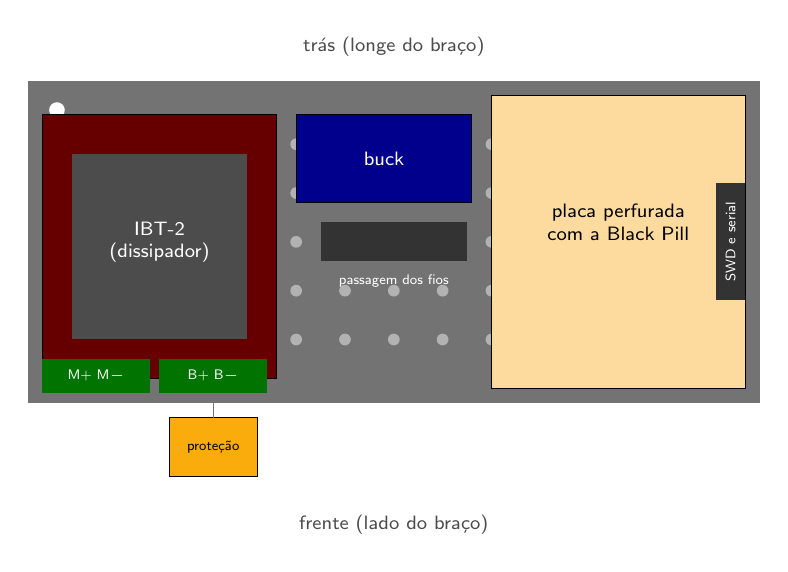
\begin{tikzpicture}[il, x=0.62mm, y=0.62mm]
  \fill[black!55] (-75,-33) rectangle (75,33);
  \foreach \i in {-6,...,6} \foreach \j in {-2,...,2} \fill[black!30] (\i*10,\j*10) circle (1.2);
  \foreach \sx in {-1,1} \foreach \sy in {-1,1} \fill[white] (\sx*69,\sy*27) circle (1.6);
  \fill[black!80] (-15,-4) rectangle (15,4);
  \node[white, font=\sffamily\tiny] at (0,-8) {passagem dos fios};
  % IBT-2
  \fill[red!40!black, draw=black] (-72,-28) rectangle (-24,26);
  \fill[black!70] (-66,-20) rectangle (-30,18);
  \node[white, rot] at (-48,0) {IBT-2\\(dissipador)};
  \fill[green!45!black] (-72,-31) rectangle (-50,-24);
  \node[white, font=\sffamily\tiny] at (-61,-27.5) {M+ M$-$};
  \fill[green!45!black] (-48,-31) rectangle (-26,-24);
  \node[white, font=\sffamily\tiny] at (-37,-27.5) {B+ B$-$};
  \fill[yellow!35!orange, draw=black] (-46,-48) rectangle (-28,-36);
  \node[rot, font=\sffamily\tiny] at (-37,-42) {proteção};
  \draw[guia] (-37,-36) -- (-37,-31);
  % buck
  \fill[blue!55!black, draw=black] (-20,8) rectangle (16,26);
  \node[white] at (-2,17) {buck};
  % placa perfurada
  \fill[yellow!25!orange!35, draw=black] (20,-30) rectangle (72,30);
  \node[rot] at (46,4) {placa perfurada\\com a Black Pill};
  \fill[black!80] (66,-12) rectangle (72,12);
  \node[rot, rotate=90, white, font=\sffamily\tiny] at (69,0) {SWD e serial};
  \node[rot, black!70] at (0,40) {trás (longe do braço)};
  \node[rot, black!70] at (0,-58) {frente (lado do braço)};
\end{tikzpicture}}

% ---------------------------------------------------------------------
% Nomes das partes: braço (face de trás) e base
\newcommand{\ilNomesBraco}{%
\begin{tikzpicture}[il]
  \node[anchor=south west, inner sep=0] (img) at (0,0) {\includegraphics[width=5.2cm]{braco}};
  \begin{scope}[x={(img.south east)}, y={(img.north west)}]
    \draw[guia] (0.22,0.55) -- (-0.12,0.72) node[left, align=right] {tubo dos\\rolamentos\\(pivô)};
    \draw[guia] (0.12,0.10) -- (-0.12,0.18) node[left, align=right] {cauda: bate\\nos batentes};
    \draw[guia] (0.70,0.80) -- (1.08,0.95) node[right, align=left] {rebaixo onde\\encaixa o motor};
    \draw[guia] (0.62,0.86) -- (1.08,0.72) node[right, align=left] {2 furos M4\\do motor};
    \draw[guia] (0.38,0.66) -- (1.08,0.50) node[right, align=left] {2 insertos\\do MPU6050};
    \draw[guia] (0.48,0.61) -- (1.08,0.50);
  \end{scope}
\end{tikzpicture}}

\newcommand{\ilNomesBase}{%
\begin{tikzpicture}[il]
  \node[anchor=south west, inner sep=0] (img) at (0,0) {\includegraphics[width=7.4cm]{etapa6_base}};
  \begin{scope}[x={(img.south east)}, y={(img.north west)}]
    \draw[guia] (0.40,0.52) -- (0.30,1.10) node[above, align=center] {suportes da barra\\(frente e trás)};
    \draw[guia] (0.50,0.80) -- (0.30,1.10);
    \draw[guia] (0.67,0.82) -- (0.78,1.10) node[above, align=center] {bandeja nas\\4 colunas};
    \draw[guia] (0.22,0.50) -- (-0.08,0.70) node[left, align=right] {batentes, com\\as almofadas};
    \draw[guia] (0.66,0.42) -- (-0.08,0.70);
    \draw[guia] (0.08,0.35) -- (-0.08,0.25) node[left, align=right] {postes da\\proteção};
    \draw[guia] (0.62,0.17) -- (-0.08,0.25);
    \node[below, align=center] at (0.5,-0.02) {frente (lado da roda) para baixo e à esquerda};
  \end{scope}
\end{tikzpicture}}
